\documentclass[sigconf,nonacm]{acmart}

\settopmatter{printacmref=false,printccs=false,printfolios=true}
\renewcommand\footnotetextcopyrightpermission[1]{}
\pagestyle{plain}

\usepackage{amsmath}
\usepackage{booktabs}
\usepackage{graphicx}
\usepackage{microtype}
\usepackage{multirow}
\usepackage{placeins}
\usepackage{subcaption}
\usepackage{tikz}
\usepackage{pgfplots}
\usepackage{xcolor}
\usepackage{xurl}
\usetikzlibrary{arrows.meta,fit,positioning}
\pgfplotsset{compat=1.18}

\definecolor{encoderblue}{HTML}{DCEAF7}
\definecolor{adaptergold}{HTML}{F6E8C3}
\definecolor{npagreen}{HTML}{DDEEDB}
\definecolor{renderred}{HTML}{F3D8D4}
\definecolor{systemgray}{HTML}{E8E9EB}
\definecolor{plotblue}{HTML}{2C6EAA}
\definecolor{plotred}{HTML}{B4463A}
\definecolor{plotgreen}{HTML}{3A7D44}

\graphicspath{{figures/}}
\newcommand{\npa}{\mathrm{NPA}}
\newcommand{\hypernpa}{\mathrm{HyperNPA}}
\newcommand{\figroot}{.}
\newcommand{\particles}{particle\nobreakdash-steps}

\title{HyperNPA: Amortized Image-Conditioned Neural Particle Automata with Spatial Token Adapters}

\author{Mitchell Mosure}
\email{mitchell@mosure.me}
\affiliation{%
  \institution{Independent Research}
  \city{Remote}
  \country{USA}
}

\begin{abstract}
Neural Particle Automata (NPA) encode a morphology in a compact local update
rule, but existing morphogenesis results train one rule per target. We study
\emph{HyperNPA}: feed-forward generation of a target-specific NPA controller
from a single RGBA image. A frozen DINOv2 ViT-S/14 preserves its class token
and $16\!\times\!16$ patch grid; a module-aware cross-attention hypernetwork
maps these 257 spatial tokens to identifiable full-rank deltas for a shared
10.9k-parameter NPA; and gradients from an alpha-aware differentiable particle
rollout train the shared rule and generator end-to-end. We implement the full
path in Rust with Burn and device-side tiled perception and splatting adjoints.

We introduce a leakage-safe evaluation protocol that separates released
target-specific NPA oracles, non-amortized per-identity adapter controls, and
identity-disjoint image-conditioned inference. On a deterministic
OmniSVG-1k split, the selected model obtains 11.63 dB aggregate composited
PSNR and 9.32 dB p10 at 2,048 particles and 1,024 steps; correct conditioning
adds 2.79 dB over shuffled images and generated deltas add 3.26 dB over the
shared base. A historical 16-target direct-adapter run reached 23.58 dB, but
used a per-image output bias absent from the released Growing NPA and is
excluded from parity claims. On two strictly held-out targets with
released NPA checkpoints, HyperNPA obtains 9.63--11.65 dB versus
27.45--27.93 dB for target-specific oracles. Dense 4,096-particle renderer
captures expose failures that white-background PSNR can obscure, including
coarse silhouettes, color-only matches, and collapsed particle masses. These
results establish an auditable end-to-end baseline and conditional
controllability, but not oracle-quality generalization. The maintained trainer
now includes a conditional row-flow generator; no row-flow quality is
retroactively attributed to the deterministic checkpoint evaluated here.
\end{abstract}

\keywords{neural particle automata, hypernetworks, self-organization,
particle systems, morphogenesis, amortized adaptation}

\begin{teaserfigure}
  \centering
  \setlength{\tabcolsep}{2pt}
  \begin{tabular}{cccccc}
    \scriptsize Rose target & \scriptsize HyperNPA & \scriptsize Oracle &
    \scriptsize Fish target & \scriptsize HyperNPA & \scriptsize Oracle \\
    
\includegraphics[width=.155\textwidth]{\figroot/targets/catalog_rose.png} &
    
\includegraphics[width=.155\textwidth]{\figroot/catalog/hyper_rose/hyper_rose_step001024.png} &
    
\includegraphics[width=.155\textwidth]{\figroot/catalog/oracle_rose/oracle_rose_step001024.png} &
    
\includegraphics[width=.155\textwidth]{\figroot/targets/catalog_tropical_fish.png} &
    
\includegraphics[width=.155\textwidth]{\figroot/catalog/hyper_tropical_fish/hyper_tropical_fish_step001024.png} &
    
\includegraphics[width=.155\textwidth]{\figroot/catalog/oracle_tropical_fish/oracle_tropical_fish_step001024.png}
  \end{tabular}
  \caption{Same-target, same-seed, 4,096-particle rollouts at step 1,024.
  HyperNPA receives each target only as a held-out condition image; the oracle
  is the released independently trained target-specific NPA. All particle
  images are unmodified captures from the Bevy/WGPU Gaussian-splatting
  renderer. HyperNPA recovers coarse color and occupancy but not the oracle's
  morphology.}
  \Description{Two target images, a rose and a tropical fish, each followed by
  a coarse held-out HyperNPA particle rendering and a recognizable rendering
  from the released target-specific NPA oracle.}
  \label{fig:teaser}
\end{teaserfigure}

\begin{document}
\maketitle

\section{Introduction}

Neural Cellular Automata learn a shared local rule whose repeated application
produces global structure~\cite{mordvintsev2020growing}. Neural Particle
Automata (NPA) move this principle from a static grid to a Lagrangian particle
system: particles carry continuous positions and latent states, perceive local
neighbors through differentiable smoothed-particle-hydrodynamics (SPH)
operators, and repeatedly apply a small shared MLP~\cite{kim2026npa}. The
released NPA models form detailed, persistent morphologies with only about
11k learned parameters. The cost is specialization: each target image is
optimized into a separate dynamical rule.

This work asks whether that optimization can be amortized. Given an unseen
image $c$, can one feed-forward network emit a controller that makes a shared
particle substrate self-organize into $c$? This is more demanding than direct
image synthesis. The generated weights must induce useful local communication,
transport thousands of particles from an unstructured seed, assign color, and
remain stable under hundreds of recurrent updates.

Hypernetworks provide a natural mechanism for condition-dependent
weights~\cite{ha2016hypernetworks}, while LoRA-style factorizations provide a
convenient adapter contract~\cite{hu2021lora}. However, three ambiguities make
an apparently strong result easy to misinterpret. First, a per-identity
adapter table is a capacity control, not an image-conditioned model. Second,
regressing non-identifiable LoRA factors can reward coordinate agreement
without functional agreement. Third, whole-image PSNR on transparent assets
can be dominated by empty background. We therefore build the study around
functional rollout loss, canonical weight deltas, identity-disjoint splits,
condition-shuffle and shared-base controls, tail metrics, long horizons, and
actual renderer captures.

Our contributions are:
\begin{itemize}
  \item an end-to-end image-to-NPA architecture that preserves all DINOv2
  spatial tokens and generates module-structured controller deltas;
  \item a Burn-native GPU path for independent per-image rollouts, with
  resident data and tiled perception and splatting adjoints;
  \item a strict evaluation hierarchy separating released per-target oracles,
  direct-adapter memorization controls, and held-out amortized inference; and
  \item a reproducible negative result: conditional control is active and
  temporally stable, but broad HyperNPA quality remains far below independent
  NPA oracles, with evidence locating the dominant gap in the shared recurrent
  substrate and its training objective.
\end{itemize}

\paragraph{Revision and artifact boundary.}
This manuscript was refreshed on July 26, 2026. Its numerical quality claims
remain attached to the serialized
\path{module_token_cross_attention_lora_v2} checkpoint. The maintained source
tree additionally implements a versioned conditional row-flow architecture
with noisy controller sources, a timestep-conditioned velocity transformer,
and a deterministic Heun solve. That path has passed bounded controllability
and throughput checks, but no identity-disjoint 1k/10k quality run has
established oracle parity. We therefore describe it only as post-study
implementation status in Appendix~\ref{app:row-flow}, not as a relabeling of
the measured model.

\section{Background and Related Work}

\paragraph{Neural automata.}
Growing NCA demonstrated that differentiable local rules can grow and repair
images from a seed~\cite{mordvintsev2020growing}. Isotropic variants remove
grid orientation cues~\cite{mordvintsev2022isotropic}. NPA instead represents
each cell as a moving particle and replaces grid convolution with compact SPH
perception~\cite{kim2026npa}. This concentrates computation where particles
exist and naturally supports varying discretizations. Our NPA state, update
rule, stochastic mask, seed, and SPH feature contract follow the released
growing-2D formulation; our contribution is conditional controller generation
and its evaluation.

\paragraph{Hypernetworks and adapters.}
Hypernetworks generate parameters for another network and can be optimized
through the downstream task~\cite{ha2016hypernetworks}. LoRA writes an update
as $\Delta W=(\alpha/r)BA$~\cite{hu2021lora}. Raw factors are non-identifiable:
$BA=(BR)(R^{-1}A)$ for any invertible $R$. We use the LoRA artifact and runtime
contract, but fix one factor to an identity embedding at full rank. The
conditioner therefore predicts the identifiable entries of $\Delta W$ and
bias deltas directly. This is a full-capacity controller test, not a
parameter-efficient low-rank claim.

\paragraph{Visual conditions.}
DINOv2 produces general-purpose visual features with a ViT patch
representation~\cite{oquab2024dinov2}. At $224^2$ resolution, ViT-S/14 emits
one class token and 256 patch tokens of width 384. Rather than average these
tokens, HyperNPA preserves the grid so adapter modules can attend to layout.
We use rasterized illustrations from MMSVG-Illustration, a subset associated
with the MMSVG-2M collection introduced by OmniSVG~\cite{yang2025omnisvg}.

\section{Method}

\subsection{Growing Neural Particle Automaton}

Each particle $i$ has position $x_i^t\in\mathbb{R}^2$ and state
$s_i^t\in\mathbb{R}^{16}$. Within support radius $\epsilon=0.1$, SPH operators
form the perception vector
\begin{equation}
z_i^t=\left[s_i^t,\;\widetilde{s}_i^t,\;\nabla s_i^t,\;\nabla\rho_i^t\right]
\in\mathbb{R}^{66},
\label{eq:perception}
\end{equation}
where vector gradients receive the logarithmic normalization used by
NPA~\cite{kim2026npa}. A shared two-layer MLP predicts position and state
increments:
\begin{align}
u_i^t &= W_2(c)\,\mathrm{ReLU}\!\left(W_1(c)z_i^t+b_1(c)\right)+b_2(c),\\
\Delta x_i^t &= \alpha\epsilon\,
  \frac{u_{i,1:2}^t}{1+\lVert u_{i,1:2}^t\rVert_2},\qquad
\Delta s_i^t=u_{i,3:18}^t,
\end{align}
with width 128 and $\alpha=0.5$. Positions are detached inside perception, as
in the released dynamic-particle recipe, while state gradients remain active.
A Bernoulli mask $m_i^t\sim\mathrm{Bernoulli}(0.5)$ applies asynchronous Euler
updates. The base controller contains
$128\cdot66+128+18\cdot128+18=10{,}898$ parameters.

\subsection{Image Condition Tokens}

The RGBA condition is resized to $224\times224$. Frozen DINOv2 ViT-S/14 runs
without an autodiff graph and returns $257\times384$ features. We append
patch-aligned RGB scaled by four and alpha scaled by one, obtaining
\begin{equation}
Z_c\in\mathbb{R}^{257\times388}.
\end{equation}
The class token receives image-level RGB/alpha summaries; the remaining tokens
retain the $16\times16$ patch layout. During the 1k experiment, all token
tensors occupy 0.371 GiB and remain device resident. DINO executes in bounded
batches of 64 during staging and is never differentiated.

\subsection{Module-Structured Adapter Generator}

For each adapter chunk $q$, a learned module/rank query attends to every token:
\begin{align}
e_j &= \mathrm{ReLU}(Z_{c,j}W_e+b_e),\\
a_{qj} &= \mathrm{softmax}_j\!\left(d^{-1/2}q_q^\top e_j\right),\\
h_q &= \mathrm{ReLU}\!\left(q_q+\sum_j a_{qj}e_j\right),\\
v_q &= W_o h_q+b_{o,q}.
\label{eq:adapter-generator}
\end{align}
The evaluated 1k checkpoint uses architecture v2: one dot-product attention
map per 256-coordinate chunk, hidden width 256, and one deterministic
generation step. It has 316,928 trainable parameters. The current v3 code
partitions the hidden representation into four attention heads; Section
\ref{sec:throughput} benchmarks that implementation, but we do not substitute
its training loss for the held-out quality result.

The rank-82 artifact layout contains 28,026 factor coordinates. In canonical
mode one factor for each matrix is a fixed identity embedding, only the
coordinates needed for the dense matrix delta are trainable, and both bias
deltas are generated. Thus the effective conditional output is exactly 10,898
identifiable values:
\begin{equation}
W_\ell(c)=W_\ell^{(0)}+\Delta W_\ell(c),\qquad
b_\ell(c)=b_\ell^{(0)}+\Delta b_\ell(c).
\end{equation}
The terminology ``LoRA'' describes serialization and application; the tested
rank is deliberately full-capacity. Despite historical artifact names, this
one-step deterministic decoder is \emph{not} rectified flow. A flow model
would require noisy adapter states, timestep-conditioned velocity training,
and multi-step sampling, none of which is used in the reported model.

\begin{figure*}[t]
\centering
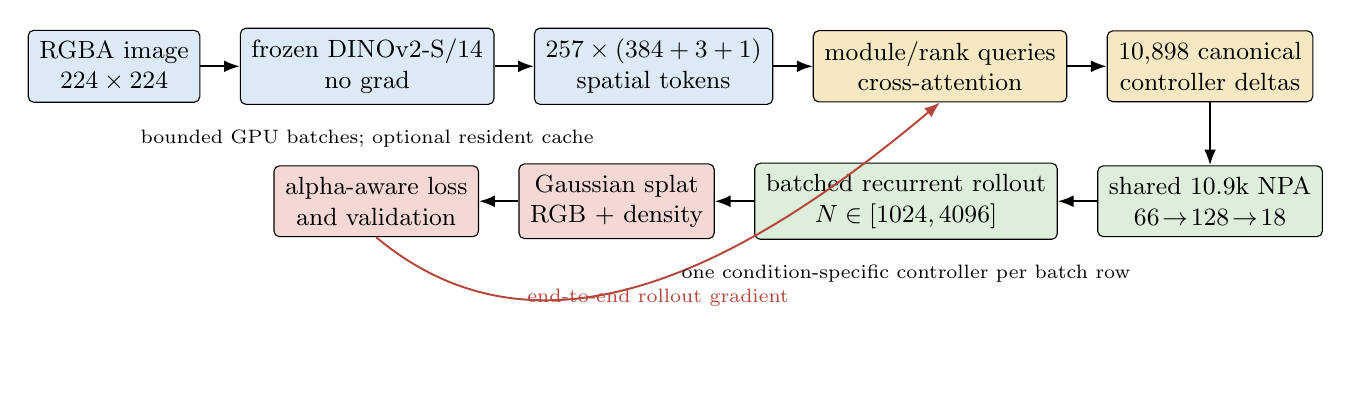
\begin{tikzpicture}[
  node distance=4mm and 5mm,
  box/.style={draw,rounded corners=2pt,minimum height=9mm,align=center,font=\small,inner sep=4pt},
  flow/.style={-{Latex[length=2mm]},line width=.7pt},
  note/.style={font=\scriptsize,align=center}
]
\node[box,fill=encoderblue] (image) {RGBA image\\$224\times224$};
\node[box,fill=encoderblue,right=of image] (dino) {frozen DINOv2-S/14\\no grad};
\node[box,fill=encoderblue,right=of dino] (tokens) {$257\times(384+3+1)$\\spatial tokens};
\node[box,fill=adaptergold,right=of tokens] (query) {module/rank queries\\cross-attention};
\node[box,fill=adaptergold,right=of query] (delta) {$10{,}898$ canonical\\controller deltas};
\node[box,fill=npagreen,below=8mm of delta] (npa) {shared 10.9k NPA\\$66\!\to\!128\!\to\!18$};
\node[box,fill=npagreen,left=of npa] (rollout) {batched recurrent rollout\\$N\in[1024,4096]$};
\node[box,fill=renderred,left=of rollout] (splat) {Gaussian splat\\RGB + density};
\node[box,fill=renderred,left=of splat] (loss) {alpha-aware loss\\and validation};
\draw[flow] (image)--(dino);
\draw[flow] (dino)--(tokens);
\draw[flow] (tokens)--(query);
\draw[flow] (query)--(delta);
\draw[flow] (delta)--(npa);
\draw[flow] (npa)--(rollout);
\draw[flow] (rollout)--(splat);
\draw[flow] (splat)--(loss);
\draw[flow,plotred] (loss.south) to[out=-40,in=-140] node[note,below]{end-to-end rollout gradient} (query.south);
\node[note,below=2mm of dino] {bounded GPU batches; optional resident cache};
\node[note,below=2mm of rollout] {one condition-specific controller per batch row};
\end{tikzpicture}
\caption{HyperNPA training and inference. The image encoder is frozen. The
conditioner and, in the selected refinement, the shared NPA base receive
gradients only through the rendered recurrent rollout objective. Evaluation
materializes the generated controller once, then uses the same NPA inference
path as released target-specific models.}
\Description{Pipeline diagram from an RGBA image through frozen DINO spatial
tokens and a module-aware adapter generator into a shared NPA, recurrent
particle rollout, Gaussian splatting, and an end-to-end image loss.}
\label{fig:architecture}
\end{figure*}

\subsection{End-to-End Rollout Training}

Each optimizer batch contains eight independent condition images and eight
independent particle trajectories. The selected refinement uses 1,024
particles, samples $T\sim[32,96]$, applies full backpropagation through time,
and maintains eight persistent pool states per training identity. Every four
optimizer steps, two pool slots per selected identity are reset to the
uniform-circle seed; live-particle-centered brush damage has radius 0.1.

Particles are centered to the target and splatted onto a $128^2$ grid with
unit-pixel Gaussian width. The last three state channels, shifted by 0.5, are
particle colors. Let $C,D$ and $C^\star,D^\star$ denote premultiplied color and
density. The training objective is
\begin{equation}
\begin{aligned}
\mathcal{L}_{\rm image}
  &=5\mathcal{L}_{\rm color}+\mathcal{L}_{\rm density}
    +10\mathcal{L}_{\rm comp},\\
\mathcal{L}
  &=2\mathcal{L}_{\rm image}+0.01\mathcal{L}_{\rm disp}\\
  &\quad+100\mathcal{L}_{\rm bound}+100\mathcal{L}_{\rm overflow}.
\end{aligned}
\label{eq:loss}
\end{equation}
$\mathcal{L}_{\rm color}$ and $\mathcal{L}_{\rm density}$ use the released
$\ell_1+\ell_2$ form; color is multiplied by a detached density-error gate so
shape is learned before appearance. $\mathcal{L}_{\rm comp}$ is squared error
after alpha compositing over white. No adapter teacher loss is used. Adam uses
generator and base learning rates $5\!\times\!10^{-5}$ and
$5\!\times\!10^{-6}$, cosine decay to $0.25\times$, per-parameter gradient
normalization, and unit-norm clipping. The 2,500-step refinement is warm
started from the preceding canonical module-decoder run.

\subsection{GPU Implementation}

Training is implemented in Burn~\cite{burnsoftware}. Conditions, target
splats, recurrent pools, generated adapters, and optimizer state remain on the
GPU. CubeCL kernels provide tiled forward and explicit vector-Jacobian product
operators for SPH perception and Target2D splatting; their adjoints have parity
tests against the dense Burn objective. Per-sample adapter application retains
the image batch dimension throughout both MLP matrices. CUDA and WGPU share
the trainer and objective; only backend dispatch and kernels differ. Bevy
inference materializes the adapter once and runs the optimized NPA hot path;
headless figures use the same WGPU simulation and Gaussian-splatting renderer
as the interactive viewer~\cite{bevysoftware,bevygaussianssoftware}.

\section{Evaluation Protocol}

\subsection{Data and Splits}

\paragraph{OmniSVG-1k.}
We use the first 1,000 cached MMSVG-Illustration training images. A deterministic
identity split assigns every tenth item to holdout (offset zero), producing 900
train and 100 holdout identities. The fixed quality subset contains 16 holdout
identities. No holdout image carries a teacher or direct adapter; the loader
aborts if this invariant is violated.

\paragraph{Released NPA catalog.}
Ten official growing-2D targets and checkpoints are imported from the released
NPA implementation~\cite{npacode}. The strict catalog experiment trains its
conditioner on eight identities and holds out \emph{rose} and
\emph{tropical fish}. These two official checkpoints provide the only
same-target independent NPA oracle comparison in this study. The lizard
checkpoint is reported as a renderer/reference sanity check, not a paired
HyperNPA holdout.

\subsection{Baselines and Controls}

\begin{table}[t]
\caption{Evaluation hierarchy. ``Train'' rows cannot establish image
generalization.}
\label{tab:evaluation-hierarchy}
\centering
\resizebox{\columnwidth}{!}{%
\begin{tabular}{llll}
\toprule
Controller & Condition & Split & Purpose \\
\midrule
Released NPA & target-specific optimization & target & oracle \\
Direct table & sample ID & train & substrate ceiling \\
Shared base & none & holdout & unconditional control \\
Shuffled HyperNPA & wrong image & holdout & condition control \\
HyperNPA & unseen image & holdout & amortized model \\
Target splat & target points & holdout & renderer ceiling \\
\bottomrule
\end{tabular}
}
\end{table}

The \emph{direct table} selects one canonical dense-delta row per training
identity and bypasses DINO and the hypernetwork. It tests whether a shared base
plus adapters can fit multiple targets under the same recurrent objective. It
is not a generalized model and is never called an oracle. The \emph{target
splat} directly renders the extracted 4,096 target points and bounds losses
caused by target preprocessing, particle count, and splat resolution.

\subsection{Metrics}

Numerical validation uses the differentiable Target2D renderer. For MSE $e$ on
unit-range values, $\mathrm{PSNR}=-10\log_{10}e$. We report:
\begin{itemize}
  \item \textbf{composited RGB PSNR}, on $C+(1-D)\mathbf{1}$;
  \item \textbf{foreground RGB PSNR}, on straight RGB weighted only by target
  foreground occupancy;
  \item \textbf{density PSNR} after clamping $D,D^\star$ to $[0,1]$;
  \item \textbf{density soft IoU},
  $\sum\min(D,D^\star)/\sum\max(D,D^\star)$;
  \item \textbf{p10 and minimum PSNR}, exposing the low-quality tail;
  \item \textbf{condition gap}, correct minus shuffled-condition PSNR; and
  \item \textbf{adapter gain}, generated-controller minus base PSNR.
\end{itemize}
The quality checkpoint is selected by the minimum p10 over horizons of at
least 256 steps, rather than training loss or mean PSNR. White-background
composited PSNR can favor sparse images and cannot substitute for foreground,
density, IoU, and visual evidence.

\subsection{Common Rollout Contract}

Unless stated otherwise, validation starts from a uniform circle of radius
0.2, uses seed 42, update probability 0.5, and horizons
$T\in\{96,256,512,1024\}$. OmniSVG numerical validation uses 2,048 particles;
the target-splat ceiling uses 4,096 extracted points. Catalog numerical
validation and every paper screenshot use 4,096 particles. Screenshots are
raw $512^2$ Bevy/WGPU captures with a black viewer background; reported PSNR
comes from the alpha-aware differentiable renderer, not screenshot pixels.

\section{Results}

\subsection{Strict Released-Oracle Comparison}

\begin{table}[t]
\caption{Strict same-target catalog comparison at 4,096 particles and 1,024
steps. Oracle checkpoints are released target-specific NPA models; HyperNPA
never saw either target or adapter during training.}
\label{tab:catalog}
\centering
\small
\begin{tabular}{llrrrr}
\toprule
Target & Controller & Comp. & Fore. & Dens. & IoU \\
\midrule
Rose & HyperNPA & 9.63 & 8.85 & 7.78 & .403 \\
Rose & released oracle & \textbf{27.93} & \textbf{27.57} & \textbf{26.89} & \textbf{.970} \\
Fish & HyperNPA & 11.65 & 10.31 & 8.46 & .593 \\
Fish & released oracle & \textbf{27.45} & \textbf{26.65} & \textbf{26.61} & \textbf{.970} \\
\midrule
Lizard & released oracle & 21.08 & 24.51 & 19.07 & .881 \\
\bottomrule
\end{tabular}
\end{table}

HyperNPA trails the paired oracle by 18.30 dB on rose and 15.80 dB on fish.
Its two-target aggregate is 10.52 dB, foreground PSNR is 9.52 dB, density PSNR
is 8.11 dB, and mean IoU is 0.498. The generated controller adds 2.33 dB over
the shared base, but the correct-over-shuffled gap is only 0.09 dB. Figure
\ref{fig:catalog-rollouts} shows that the controller recovers broad hue and
occupancy while missing target topology. The released controllers form the
expected shapes and remain coherent at step 1,024.

\begin{figure*}[t]
\centering
\setlength{\tabcolsep}{2pt}
\begin{tabular}{c@{\hspace{4pt}}cc@{\hspace{7pt}}cc}
& \multicolumn{2}{c|}{HyperNPA} & \multicolumn{2}{c}{Released oracle} \\
Target & $T=96$ & $T=1024$ & $T=96$ & $T=1024$ \\

\includegraphics[width=.16\textwidth]{\figroot/targets/catalog_rose.png} &

\includegraphics[width=.16\textwidth]{\figroot/catalog/hyper_rose/hyper_rose_step000096.png} &

\includegraphics[width=.16\textwidth]{\figroot/catalog/hyper_rose/hyper_rose_step001024.png} &

\includegraphics[width=.16\textwidth]{\figroot/catalog/oracle_rose/oracle_rose_step000096.png} &

\includegraphics[width=.16\textwidth]{\figroot/catalog/oracle_rose/oracle_rose_step001024.png} \\

\includegraphics[width=.16\textwidth]{\figroot/targets/catalog_tropical_fish.png} &

\includegraphics[width=.16\textwidth]{\figroot/catalog/hyper_tropical_fish/hyper_tropical_fish_step000096.png} &

\includegraphics[width=.16\textwidth]{\figroot/catalog/hyper_tropical_fish/hyper_tropical_fish_step001024.png} &

\includegraphics[width=.16\textwidth]{\figroot/catalog/oracle_tropical_fish/oracle_tropical_fish_step000096.png} &

\includegraphics[width=.16\textwidth]{\figroot/catalog/oracle_tropical_fish/oracle_tropical_fish_step001024.png}
\end{tabular}
\caption{Held-out catalog rollouts under a common 4,096-particle contract.
The comparison holds target, seed, asynchronous update probability, renderer,
and horizon fixed.}
\Description{Rose and tropical-fish targets followed by HyperNPA and released
oracle particle rollouts at 96 and 1024 steps. The oracle forms recognizable
targets while HyperNPA produces coarse colored masses.}
\label{fig:catalog-rollouts}
\end{figure*}

\subsection{Identity-Disjoint OmniSVG-1k}

\begin{table}[t]
\caption{Selected OmniSVG-1k holdout result at 2,048 particles. Aggregate
metrics pool pixel MSE before converting to PSNR; p10 is over 16 identities.}
\label{tab:omnisvg-main}
\centering
\small
\begin{tabular}{lr}
\toprule
Metric at $T=1024$ & Result \\
\midrule
Aggregate composited RGB PSNR & 11.63 dB \\
Mean / p10 / minimum PSNR & 12.70 / 9.32 / 8.30 dB \\
Aggregate foreground RGB PSNR & 9.56 dB \\
Aggregate density PSNR & 8.77 dB \\
Mean density soft IoU & 0.536 \\
Correct condition over shuffled & 2.79 dB \\
Generated controller over shared base & 3.26 dB \\
Target-point-splat p10 ceiling & 28.08 dB \\
Gap to target-point-splat p10 & 18.77 dB \\
\bottomrule
\end{tabular}
\end{table}

Table~\ref{tab:omnisvg-main} proves that both condition and generated adapter
paths affect held-out behavior. It also rejects particle extraction as the
primary explanation: the same targets can be splatted above 28 dB p10. Yet
all 16 examples miss the 26 dB gate and pairwise generated adapters remain
similar (mean cosine 0.992), consistent with an overly unconditional shared
attractor.

\begin{figure}[t]
\centering
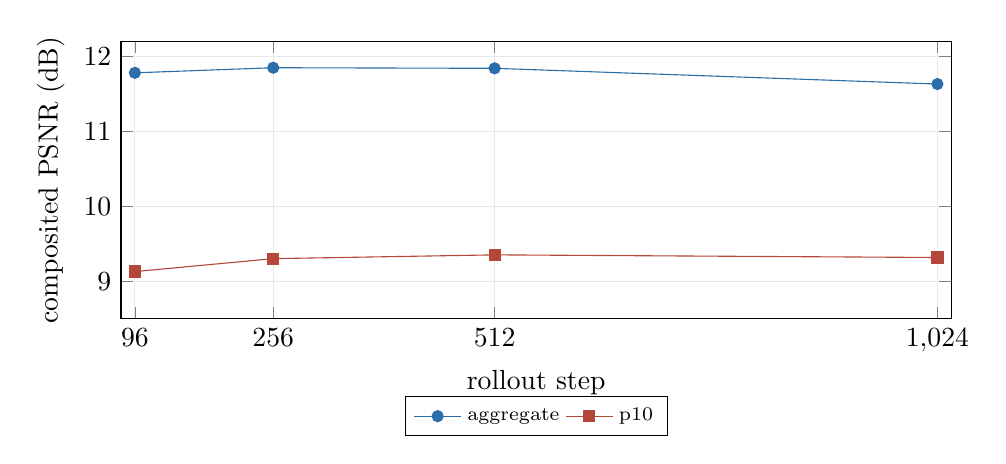
\begin{tikzpicture}
\begin{axis}[
  width=\columnwidth,height=5.1cm,
  xlabel={rollout step},ylabel={composited PSNR (dB)},
  xmin=80,xmax=1040,ymin=8.5,ymax=12.2,
  xtick={96,256,512,1024},
  legend style={font=\scriptsize,at={(0.5,-0.28)},anchor=north,legend columns=2},
  grid=major,grid style={systemgray}
]
\addplot[color=plotblue,mark=*] coordinates {(96,11.7833) (256,11.8515) (512,11.8436) (1024,11.6334)};
\addlegendentry{aggregate}
\addplot[color=plotred,mark=square*] coordinates {(96,9.1288) (256,9.3015) (512,9.3521) (1024,9.3169)};
\addlegendentry{p10}
\end{axis}
\end{tikzpicture}
\caption{The selected 1k checkpoint is dynamically stable but stably
low-quality. Peak-to-final p10 loss is only 0.035 dB; more inference steps do
not close the quality gap.}
\Description{Line chart showing nearly flat aggregate and tenth-percentile
composited PSNR from 96 through 1024 rollout steps.}
\label{fig:horizons}
\end{figure}

\begin{figure}[t]
\centering
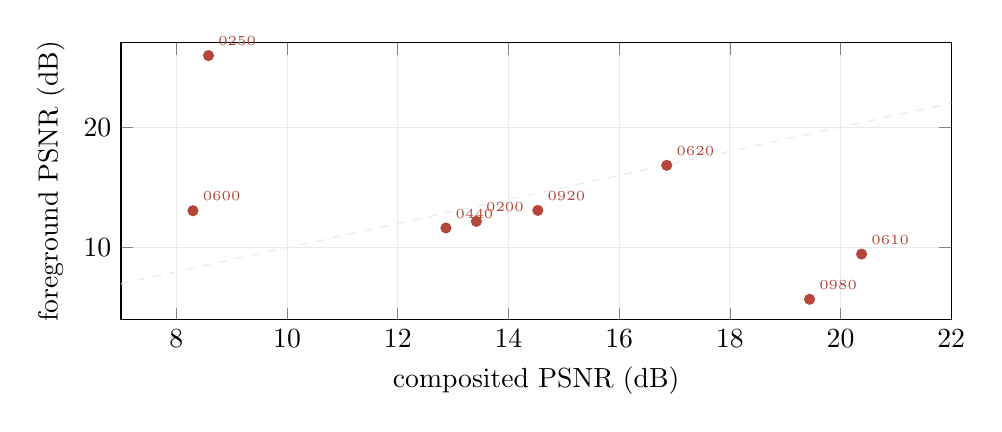
\begin{tikzpicture}
\begin{axis}[
  width=\columnwidth,height=5.1cm,
  xlabel={composited PSNR (dB)},ylabel={foreground PSNR (dB)},
  xmin=7,xmax=22,ymin=4,ymax=27,
  grid=major,grid style={systemgray},
  nodes near coords,
  point meta=explicit symbolic,
  every node near coord/.append style={font=\tiny,anchor=south west}
]
\addplot[color=systemgray,dashed,domain=7:22,samples=2] {x};
\addplot[only marks,mark=*,color=plotred,mark size=1.8pt]
coordinates {
  (20.38,9.46) [0610]
  (19.44,5.71) [0980]
  (16.86,16.83) [0620]
  (14.53,13.09) [0920]
  (13.42,12.18) [0200]
  (12.87,11.63) [0440]
  (8.58,25.94) [0250]
  (8.30,13.06) [0600]
};
\end{axis}
\end{tikzpicture}
\caption{Whole-image composited PSNR and alpha-weighted foreground PSNR can
disagree sharply. IDs correspond to Figure~\ref{fig:omnisvg-rollouts}.}
\Description{Scatter plot of composited versus foreground PSNR for eight
held-out images. Several points lie far from the equal-score diagonal.}
\label{fig:metric-disagreement}
\end{figure}

\begin{figure*}[t]
\centering
\setlength{\tabcolsep}{2pt}
\scriptsize
\begin{tabular}{c@{\hspace{3pt}}cccc}
Condition & Target & $T=96$ & $T=256$ & $T=1024$ \\
0610 (20.38 dB) &

\includegraphics[width=.131\textwidth]{\figroot/targets/heldout_0610.png} &

\includegraphics[width=.131\textwidth]{\figroot/heldout/00000610_e79c37971204e6ffdaa53d7aa1eea84a/00000610_e79c37971204e6ffdaa53d7aa1eea84a_step000096.png} &

\includegraphics[width=.131\textwidth]{\figroot/heldout/00000610_e79c37971204e6ffdaa53d7aa1eea84a/00000610_e79c37971204e6ffdaa53d7aa1eea84a_step000256.png} &

\includegraphics[width=.131\textwidth]{\figroot/heldout/00000610_e79c37971204e6ffdaa53d7aa1eea84a/00000610_e79c37971204e6ffdaa53d7aa1eea84a_step001024.png} \\
0980 (19.44 dB) &

\includegraphics[width=.131\textwidth]{\figroot/targets/heldout_0980.png} &

\includegraphics[width=.131\textwidth]{\figroot/heldout/00000980_5f7c045634a05e6bdbeceb040deb0012/00000980_5f7c045634a05e6bdbeceb040deb0012_step000096.png} &

\includegraphics[width=.131\textwidth]{\figroot/heldout/00000980_5f7c045634a05e6bdbeceb040deb0012/00000980_5f7c045634a05e6bdbeceb040deb0012_step000256.png} &

\includegraphics[width=.131\textwidth]{\figroot/heldout/00000980_5f7c045634a05e6bdbeceb040deb0012/00000980_5f7c045634a05e6bdbeceb040deb0012_step001024.png} \\
0620 (16.86 dB) &

\includegraphics[width=.131\textwidth]{\figroot/targets/heldout_0620.png} &

\includegraphics[width=.131\textwidth]{\figroot/heldout/00000620_ddb3fc487a832a1a1c346f31ac5c26d1/00000620_ddb3fc487a832a1a1c346f31ac5c26d1_step000096.png} &

\includegraphics[width=.131\textwidth]{\figroot/heldout/00000620_ddb3fc487a832a1a1c346f31ac5c26d1/00000620_ddb3fc487a832a1a1c346f31ac5c26d1_step000256.png} &

\includegraphics[width=.131\textwidth]{\figroot/heldout/00000620_ddb3fc487a832a1a1c346f31ac5c26d1/00000620_ddb3fc487a832a1a1c346f31ac5c26d1_step001024.png} \\
0920 (14.53 dB) &

\includegraphics[width=.131\textwidth]{\figroot/targets/heldout_0920.png} &

\includegraphics[width=.131\textwidth]{\figroot/heldout/00000920_de4f860c68d30a914d7812d441662bf0/00000920_de4f860c68d30a914d7812d441662bf0_step000096.png} &

\includegraphics[width=.131\textwidth]{\figroot/heldout/00000920_de4f860c68d30a914d7812d441662bf0/00000920_de4f860c68d30a914d7812d441662bf0_step000256.png} &

\includegraphics[width=.131\textwidth]{\figroot/heldout/00000920_de4f860c68d30a914d7812d441662bf0/00000920_de4f860c68d30a914d7812d441662bf0_step001024.png} \\
0200 (13.42 dB) &

\includegraphics[width=.131\textwidth]{\figroot/targets/heldout_0200.png} &

\includegraphics[width=.131\textwidth]{\figroot/heldout/00000200_b2d25a52e7685808e57b6cf8e539fa22/00000200_b2d25a52e7685808e57b6cf8e539fa22_step000096.png} &

\includegraphics[width=.131\textwidth]{\figroot/heldout/00000200_b2d25a52e7685808e57b6cf8e539fa22/00000200_b2d25a52e7685808e57b6cf8e539fa22_step000256.png} &

\includegraphics[width=.131\textwidth]{\figroot/heldout/00000200_b2d25a52e7685808e57b6cf8e539fa22/00000200_b2d25a52e7685808e57b6cf8e539fa22_step001024.png} \\
0440 (12.87 dB) &

\includegraphics[width=.131\textwidth]{\figroot/targets/heldout_0440.png} &

\includegraphics[width=.131\textwidth]{\figroot/heldout/00000440_b0247c80110d29b145be58ada2836291/00000440_b0247c80110d29b145be58ada2836291_step000096.png} &

\includegraphics[width=.131\textwidth]{\figroot/heldout/00000440_b0247c80110d29b145be58ada2836291/00000440_b0247c80110d29b145be58ada2836291_step000256.png} &

\includegraphics[width=.131\textwidth]{\figroot/heldout/00000440_b0247c80110d29b145be58ada2836291/00000440_b0247c80110d29b145be58ada2836291_step001024.png} \\
0250 (8.58 dB) &

\includegraphics[width=.131\textwidth]{\figroot/targets/heldout_0250.png} &

\includegraphics[width=.131\textwidth]{\figroot/heldout/00000250_cb66a153fb3fb03cc31943e3a147911e/00000250_cb66a153fb3fb03cc31943e3a147911e_step000096.png} &

\includegraphics[width=.131\textwidth]{\figroot/heldout/00000250_cb66a153fb3fb03cc31943e3a147911e/00000250_cb66a153fb3fb03cc31943e3a147911e_step000256.png} &

\includegraphics[width=.131\textwidth]{\figroot/heldout/00000250_cb66a153fb3fb03cc31943e3a147911e/00000250_cb66a153fb3fb03cc31943e3a147911e_step001024.png} \\
0600 (8.30 dB) &

\includegraphics[width=.131\textwidth]{\figroot/targets/heldout_0600.png} &

\includegraphics[width=.131\textwidth]{\figroot/heldout/00000600_a14bc90de0979fafe98826f2012ec410/00000600_a14bc90de0979fafe98826f2012ec410_step000096.png} &

\includegraphics[width=.131\textwidth]{\figroot/heldout/00000600_a14bc90de0979fafe98826f2012ec410/00000600_a14bc90de0979fafe98826f2012ec410_step000256.png} &

\includegraphics[width=.131\textwidth]{\figroot/heldout/00000600_a14bc90de0979fafe98826f2012ec410/00000600_a14bc90de0979fafe98826f2012ec410_step001024.png}
\end{tabular}
\caption{Eight identity-disjoint OmniSVG holdouts. Every rollout uses 4,096
particles; parenthesized metrics are the corresponding 2,048-particle
Target2D composited PSNR at $T=1024$. Even the highest-scoring building is a
coarse mass, the hearts become a wedge, and sparse line art largely
disappears. The trajectories are stable in time but not semantically faithful.}
\Description{Eight held-out target images and their 4096-particle HyperNPA
rollouts at 96, 256, and 1024 steps. Outputs preserve broad colors while
detailed shapes collapse into coarse disks, wedges, or compact masses.}
\label{fig:omnisvg-rollouts}
\end{figure*}
\FloatBarrier

\subsection{Shared-Substrate Capacity Control}

The direct adapter table removes image encoding and generation. Sixteen
training identities jointly optimize the shared base and one canonical delta
per identity under progressively denser rollouts. The campaign matches
upstream compute exposure by counting a trajectory at $N$ particles as
$N/4096$ of a 4,096-particle trajectory. The 512-, 1,024-, and 2,048-particle
stages total 250,000 equivalent trajectories per identity, or 104.17\% of the
released recipe's 240,000. All rows are evaluated at 4,096 particles.

\begin{table}[t]
\caption{Historical non-amortized 16-identity diagnostic. These runs predate
the zero-output-bias parity contract and are not valid oracle ceilings.
Throughput is median optimizer throughput.}
\label{tab:capacity}
\centering
\resizebox{\columnwidth}{!}{%
\begin{tabular}{lrrrr}
\toprule
Training continuation & Agg. & p10 & Gap & M\particles/s \\
\midrule
512p, 240k traj./ID & 13.06 & 10.82 & 4.85 & 13.26 \\
$+$1024p, 240k traj./ID & 15.87 & 13.24 & 7.79 & 10.21 \\
$+$2048p, 320k traj./ID & 20.71 & 18.05 & 12.60 & 6.90 \\
$+$4096p density cycle & 20.71 & 18.05 & 12.60 & 4.11 \\
frozen base, table refine & 23.58 & 19.30 & 15.46 & 4.03 \\
\bottomrule
\end{tabular}
}
\end{table}

Increased particle density and exposure produced large gains in this legacy
control. However, its canonical adapter trained an image-specific output bias,
whereas the released Growing NPA has no final-layer bias. The entire table is
therefore retained only as historical optimization evidence and cannot bound
the zero-bias conditioned architecture. A bounded corrected control used an
upstream-seeded shared rule, zero-output-bias rank-82 controllers, 4,096
particles, eight trajectories per identity, and rollout lengths sampled from
32--95. After 2,000 joint updates (16,000 trajectories per identity, 6.67\% of
the released exposure), it reached 11.63 dB aggregate and 10.52 dB p10 at
1,024 steps; its minimum multi-horizon p10 was 10.43 dB. Correct controllers
outperformed shuffled identities by 3.77 dB, confirming that the substrate was
active, but the result is far below parity and is not a converged capacity
ceiling. A full-exposure parity-validated control remains necessary before
attributing the gap to amortization alone.

\subsection{Metric Failure Modes}

The 16 held-out examples reveal why one score is insufficient. Condition 0610
has the highest composited PSNR (20.38 dB) but only 9.46 dB foreground PSNR;
its building becomes a colored blob. Condition 0980 obtains 19.44 dB
composited PSNR yet only 5.71 dB foreground PSNR and 0.152 IoU. Conversely,
condition 0250 has 25.94 dB foreground color PSNR but 8.58 dB composited PSNR
because it predicts approximately the right color in the wrong occupancy.
These are not numerical edge cases: Figure~\ref{fig:omnisvg-rollouts} shows
the corresponding 4,096-particle states.

\subsection{Training Throughput}
\label{sec:throughput}

The current v3 CUDA profile uses 64 independent conditions, 1,024 particles,
96 full-BPTT steps, release mode, and an NVIDIA RTX PRO 6000 Blackwell (96 GiB,
600 W). Validation and checkpoint I/O are disabled. Exact optimizer exposure
is 1.887 billion particle-steps over 300 updates.

\begin{table}[t]
\caption{Current module-token v3 systems benchmark. It demonstrates trainer
throughput, not the quality of the selected v2 checkpoint.}
\label{tab:throughput}
\centering
\resizebox{\columnwidth}{!}{%
\begin{tabular}{lr}
\toprule
Metric & Result \\
\midrule
Measured end-to-end optimizer throughput & 17.66 M\particles/s \\
Median report-window throughput & 18.36 M\particles/s \\
Minimum / maximum report window & 15.93 / 18.76 M\particles/s \\
Training wall time & 109.1 s \\
Condition batch / particle count / steps & 64 / 1024 / 96 \\
Perception custom-op device hits & 28,800 forward \\
Perception VJP device hits & 28,500 backward \\
Host perception fallbacks & 0 \\
\bottomrule
\end{tabular}
}
\end{table}

This is an $8.5\times$ increase over the selected WGPU quality refinement's
2.08 M\particles/s median, but hardware, backend, batch size, and decoder
version all change, so it is not a controlled kernel-only speedup. The profile
does establish that the current trainer can sustain tens of millions of
particle updates per second without host perception fallback. Quality-scale
4,096-particle backward remains the expensive regime.

\section{Discussion}

\subsection{What Has Been Demonstrated}

The experiments support three positive conclusions. First, per-sample
conditioned controllers are correctly batched and applied: correct images
outperform shuffled images by 2.79 dB on OmniSVG, and generated adapters
outperform the shared base by 3.26 dB. Second, the target representation and
4,096-particle renderer can express high-quality outputs: direct target splats
reach 28.08 dB p10 and released rose/fish controllers reach about 27.5 dB.
Third, conditional control, runtime materialization, and GPU training are
alive. The historical 23.58 dB table result is not counted as parity evidence
because it used a per-image output bias unavailable to the released NPA.

\subsection{What Has Not Been Demonstrated}

The present model does not achieve oracle-quality or broad high-fidelity
generalization. The primary 1k numerical result covers only 16 of 100 held-out
identities, one deterministic split, and one rollout seed. The catalog oracle
comparison covers two identities. We report no confidence intervals, no
damage-regeneration test for generated controllers, and no independently
overfit NPA oracle bank for the OmniSVG holdouts. The best visual sample is not
faithful despite a 20.38 dB composited score.

The studied decoder is deterministic, so this work makes no rectified-flow
quality claim. DINO is frozen and was not pretrained for alpha-aware vector
graphics. Static controller deltas must encode the entire target layout;
particles do not directly sample a condition field during rollout. Finally,
the Burn objective adds white-composited RGB and strong boundary terms to the
released density/color objective. These choices are explicit, but strict
upstream training parity should be established before attributing every gap to
hypernetwork architecture.

\subsection{Evidence-Based Next Steps}

The control ladder suggests the following order:
\begin{enumerate}
  \item \textbf{Establish an independent Burn oracle.} Match released target
  extraction, seed pool, $N=4096$, $T\in[32,96]$, density-gated color loss,
  damage, optimizer, and 30k iterations; compare one-step values, gradients,
  updates, and long rollouts to the released implementation.
  \item \textbf{Raise the adapter substrate tail.} Continue multi-identity
  direct-adapter training under the zero-output-bias contract with a frozen,
  parity-validated trunk and select on 4,096-particle multi-horizon p10. No
  valid 26 dB amortization ceiling has yet been established.
  \item \textbf{Distill function, then fine-tune end to end.} Warm-start the
  v3 token generator from canonical dense deltas or probe-rollout behavior,
  then optimize downstream rollout loss with the trunk frozen before a small
  joint-learning phase.
  \item \textbf{Add spatial runtime memory.} Let particles bilinearly sample a
  compact condition feature grid in addition to static controller modulation.
  This removes pressure to encode exact image layout entirely in 10.9k weights.
  \item \textbf{Only then test stochastic flow.} Train an adapter velocity
  model with noisy canonical deltas and time conditioning, then validate sampled
  controllers through the same oracle-relative rollout suite.
\end{enumerate}

\section{Conclusion}

HyperNPA converts a condition image into a runnable NPA controller in one
feed-forward pass and executes that controller through a common optimized
particle runtime. The maintained implementation preserves spatial DINO tokens,
generates identifiable module-structured deltas, trains through the actual
recurrent image objective, and exposes strict conditional and tail metrics.
At present, it is an auditable baseline rather than a solved generative model:
held-out quality is 11.63 dB aggregate and 9.32 dB p10, while released
target-specific controllers exceed 27 dB on paired targets. The direct-adapter
control shows a plausible route upward, but also establishes a hard ordering:
first validate and optimize the shared recurrent substrate, then amortize it,
and only then add a stochastic adapter generator.

\section*{Reproducibility Statement}

The repository records TOML experiment definitions, binary checkpoints, JSON
reports, deterministic split rules, seeds, and headless renderer reports. The
paper's central evidence comes from:
\begin{itemize}
  \item OmniSVG-1k: \path{artifacts/hyper2d_omnisvg_1k_dino_canonical_quality_refine/report.json};
  \item catalog holdout: \path{artifacts/hyper2d_growing_catalog_holdout2_quality_eval_p4096_s1024/report.json};
  \item historical non-parity table diagnostic: \path{artifacts/hyper2d_omnisvg_16_p4096_frozen_table_lr2e6/report.json}; and
  \item throughput: \path{artifacts/throughput_v3_p1024_s96_b64_sources64_cuda_release_fixed96_retained_vjp/report.json}.
\end{itemize}
All paper rollouts were regenerated with the headless export command, 4,096
particles, seed 42, update probability 0.5, and captures
at steps 0, 32, 96, 256, 512, and 1,024. Appendix~\ref{app:metrics} lists the
eight visualized holdout metrics.

\appendix

\section{Per-Sample Held-Out Metrics}
\label{app:metrics}

\begin{table}[t]
\caption{The eight OmniSVG holdouts visualized in
Figure~\ref{fig:omnisvg-rollouts}. Metrics use 2,048
particles and $T=1024$; figures use 4,096 particles.}
\label{tab:per-sample}
\centering
\scriptsize
\begin{tabular}{lrrrr}
\toprule
ID & Comp. & Fore. & Density & Soft IoU \\
\midrule
0610 & 20.38 & 9.46 & 12.46 & .673 \\
0980 & 19.44 & 5.71 & 13.40 & .152 \\
0620 & 16.86 & 16.83 & 10.21 & .607 \\
0920 & 14.53 & 13.09 & 8.92 & .585 \\
0200 & 13.42 & 12.18 & 10.87 & .782 \\
0440 & 12.87 & 11.63 & 10.84 & .273 \\
0250 & 8.58 & 25.94 & 7.73 & .269 \\
0600 & 8.30 & 13.06 & 8.25 & .401 \\
\bottomrule
\end{tabular}
\end{table}

\section{Artifact and Version Boundaries}

The best 1k quality checkpoint serializes architecture
\path{module_token_cross_attention_lora_v2}. The source tree's
maintained default is
\path{module_token_multihead_cross_attention_lora_v3}. We deliberately
report the architecture stored in each artifact instead of relabeling old
weights as the latest code. Likewise, historical directory names containing
\path{rectified_flow} do not establish a flow objective. The report field
\path{generator_sample_steps=1}, zero source noise, and deterministic
artifact inference define the evaluated behavior.

The imported catalog metrics evaluate released target-specific checkpoints in
the Burn quality harness; they do not claim that the current Burn trainer can
reproduce those checkpoints from scratch. The direct adapter table uses the
same NPA runtime and loss as HyperNPA, but evaluates training identities and
must not be compared as held-out generalization.

\section{Maintained Conditional Row-Flow Path}
\label{app:row-flow}

The current trainer preserves all 257 DINOv2 tokens and appends the aligned
$14\times14$ RGBA patch payload to each of the 256 patch tokens. Deterministic
seeded source rows for the two NPA affine layers are transported by a
timestep-conditioned self/cross-attention velocity network. An eight-step
Heun solve produces 10,898 identifiable controller residuals. End-to-end image
and rollout loss updates both the generated residual and shared NPA trunk.
Detached TBPTT accumulates controller-endpoint VJPs on device and contracts
them through the flow graph once per optimizer step.

This architecture is stored as version 5 inside the versioned BPK artifact
container and remains load-compatible with legacy version-4 row-flow
artifacts. Its bounded four-condition control shows active conditioning, but
its p10 quality remains far below the 26 dB target. Consequently, broad
generalized row-flow quality is an open result, not a paper conclusion.

\bibliographystyle{ACM-Reference-Format}
\bibliography{hyper_npa}

\end{document}
